







%%%%%%%%%%%%%%%%%%%%%%%%%%%%%%%%%%%%%%%%%%%%%%%%%%%%%%%%%%%%%%%%%
%%%%%%%%%%%%%%%%%%%%%%%%%%%%%%%%%%%%%%%%%%%%%%%%%%%%%%%%%%%%%%%%%
%%%%%%%%%%%%%%%%%%%%%%%%%%%%%%%%%%%%%%%%%%%%%%%%%%%%%%%%%%%%%%%%%

\begin{frame}{Subgroup contributions: Same-Sex Marriage Survey}
Analysis of US state-level support for same-sex marriage\footnote{
    Based on \textcite{lax:2009:gay,kastellec:2010:laxmrp}.}.

\begin{itemize}
    %
    \item \surcol{\textbf{Survey population:}} Five consistently-coded national polls from 2004 
        ($\surcol{\Nsur ={}\LaxNSur}$)
    \item \surcol{\textbf{Response:}}  $\y = 1$ encodes support for same-sex marriage, $\y = 0$ opposition
       or no opinion.
    \item \tarcol{\textbf{Target population:}} US Census 5\% PUMS data for CA from 2000
    %
\end{itemize}

\pause
Let's analyze this data with two methods: \textbf{MrP} and \textbf{calibration weighting} (CW).

\pause
MrP computed with \texttt{brms} \parencite{brms}:\\
{
\tiny
$$
\begin{aligned}
\y \sim{}& \texttt{logit}\Big(~\texttt{(1 | race.female) + (1 | age.cat) + 
  (1 | edu.cat) + (1 | age.edu.cat) +}
  \\{}&\qquad\quad\;\; \texttt{(1 | state) + (1 | region) + (1 | poll) +
  p.relig.full + p.kerry.full}~\Big)
\end{aligned}
$$
}
%
CW used raking on the following coarsened regressors:
({\tiny{\texttt{survey::calibrate}}} \textcite{lumley:2025:survey}):
{
\tiny
$$
\texttt{female, edu.cat, age.cat, race.wbh, race.w.female, age.edu.low}
$$
}
%
\pause
%
\begin{minipage}{0.5\textwidth}
\vspace{-1.5em}
$$
\begin{aligned}
    \textrm{Raw survey mean:} && \surcol{\meansur \y_i} ={}& \LaxYbar \\
    \textrm{Raking:} && \muhatcw ={}& \LaxRakingMu \\
    \textrm{MrP:} && \muhatmrp ={}& \LaxMrpMu\\
\end{aligned}
$$
\end{minipage}
\hfill
\begin{minipage}{0.4\textwidth}
\vspace{-1.5em}
    \pause
    \textbf{How are MrP and raking are using the data differently?}
\end{minipage}
%
%
\end{frame}





%%%%%%%%%%%%%%%%%%%%%%%%%%%%%%%%%%%%%%%%%%%%%%%%%%%%%%%%%%%%%%%%%
%%%%%%%%%%%%%%%%%%%%%%%%%%%%%%%%%%%%%%%%%%%%%%%%%%%%%%%%%%%%%%%%%
%%%%%%%%%%%%%%%%%%%%%%%%%%%%%%%%%%%%%%%%%%%%%%%%%%%%%%%%%%%%%%%%%

\begin{frame}{Same-Sex Marriage Survey Weights}

\centering

\begin{minipage}{0.7\textwidth}
\LaxWeightPlot{}        
\end{minipage}

\onslide<2->{
    What does the difference between these weights mean in terms of
    \begin{itemize}
        \item \sout{Frequentist sampling variance (standard errors)?}
        \item \sout{Covariate balance / external validity?}
        \item Subgroup contributions?
    \end{itemize}
}

\end{frame}








%%%%%%%%%%%%%%%%%%%%%%%%%%%%%%%%%%%%%%%%%%%%%%%%%%%%%%%%%%%%%%%%%
%%%%%%%%%%%%%%%%%%%%%%%%%%%%%%%%%%%%%%%%%%%%%%%%%%%%%%%%%%%%%%%%%
%%%%%%%%%%%%%%%%%%%%%%%%%%%%%%%%%%%%%%%%%%%%%%%%%%%%%%%%%%%%%%%%%

\begin{frame}[t]{Same-Sex Marriage subgroup contribution}

Note that both methods use \emph{national data} to infer public opinion \emph{in California}.

\only<2>{
\begin{block}{Question:}
    How do responses in Texas affect our estimate of public opinion in CA?
\end{block}
}


%
\only<2>{
\centering
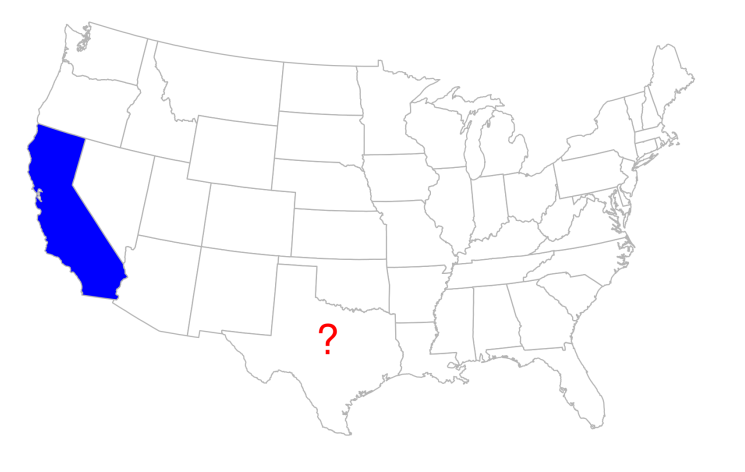
\includegraphics[width=0.5\textwidth]{static_figures/ca_query.png}
% \begin{minipage}{0.7\textwidth}
% %\MapQuery{} % Too much whitespace, include by hand
% \end{minipage}
}

\only<3->{
\begin{block}{More specific question:}
    Suppose we \emph{increased} the responses $\y_i$ in Texas.

    How would our estimate of public opinion in CA change?
\end{block}
}

\only<3>{
Take $\surcol{\ytil_i = \y_i + \delta \ind{i \textrm{ is in Texas}}}$.
%
Then $
\muhatcw[\ytil] - \muhatcw[\y] = \delta \underbrace{
        \surcol{\sum_{i \textrm{ in Texas}} \w_i}
    }_{\textrm{Texas's contribution}}$.
}

\only<4->{
Take $\surcol{\ytil_i = \y_i + \delta \ind{i \textrm{ is in Texas}}}$.
%
Then $
\muhatmrp[\ytil] - \muhatmrp[\y] \approx \delta \underbrace{
        \surcol{\sum_{i \textrm{ in Texas}} \w^\mrp_i}
    }_{\textrm{Texas's contribution}}$.
}

\begin{minipage}{0.9\textwidth}
    \centering
\only<5>{
    \LaxphilipsCAPoolingPlot{}
}
\only<6>{
    \LaxphilipsMOPoolingPlot{}
}
\end{minipage}


\end{frame}







